%! TEX root = 0-main.tex
\chapter{Geodesics}
Recall the Lagrangian
\[L = \sqrt{-g_{\mu\nu}\der{x^\mu}{\sigma}\der{x^{\nu}}{\sigma}}\]
If we work through the Euler equation,
\[0= \der{}{\sigma}\left[\pder{L}{\left(\der{x^\alpha}{\sigma}\right)}\right]-\pder{L}{x^\alpha}\]
we can find
\begin{align*}
	\pder{L}{\left(\der{x^\alpha}{\sigma}\right)} &=  \frac{1}{2}\frac{1}{\sqrt{-g_{\mu\nu}\der{x^\mu}{\sigma}\der{x^\nu}{\sigma}}}\left(-g_{\mu\nu}\delta^\mu_\alpha x^\nu - g_{\mu\nu} x^\mu \delta^\nu_\alpha\right)\\
						      &=\frac{1}{L}g_{\mu\alpha}\der{x^\mu}{\sigma}
						      \intertext{Noticing \(\der{\tau}{\sigma} = \frac{\sqrt{-g_{\mu\nu}\d{x^\mu}\d{x^\nu}}}{\sigma} = L\), we find can rewrite as}
						      &= -g_{\mu\nu}\der{x^\mu}{\tau}
\end{align*}

Similarly, we can find
\begin{align*}
	\pder{L}{x^\alpha} &= -\frac{1}{2L}\pder{g_{\mu\nu}}{x^\alpha}\der{x^\mu}{\sigma}\der{x^\nu}{\sigma}\\
			   &=-\frac{1}{2}\pder{g_{\mu\nu}}{x^\alpha}\der{x^\mu}{\tau}\der{x^\nu}{\tau}
\end{align*}
Thus, plugging into the Euler equation, we can obtain the geodesic equation
\begin{equation}
	 0 = \der{}{\tau}\left(g_{\alpha\beta}\der{x^\beta}{\tau}\right) - \frac{1}{2}\partial_{\alpha}g_{\mu\nu}\der{x^\mu}{\tau}\der{x^\nu}{\tau}
\end{equation}
Expanding the first term, we obtain
\[\der{}{\tau}\left(g_{\alpha\beta}\der{x^\beta}{\tau}\right) = \partial_\gamma g_{\alpha\beta} \der{x^\gamma}{\tau}\der{x^\beta}{\tau} + g_{\alpha\beta}\der{x^\beta}{\tau2}\]
renaming indices and multiplying by the inverse metric, we obtain 
\[0=\der{x^\gamma}{\tau} + g^{\gamma\alpha}\left(\partial_\mu g_{\alpha\nu} - \frac{1}{2}\partial_\alpha g_{\mu\nu}\right)\der{x^\mu}{\tau}\der{x^\nu}{\tau}\]
Exploiting the symmetry of
\[\partial_\mu g_{\alpha\nu}\der{x^\mu}{\tau}\der{x^\nu}{\tau} = \frac{1}{2}\left(\partial_\mu g_{\alpha\nu} + \partial_\nu g_{\alpha\mu}\right)\der{x^\mu}{\tau}\der{x^\nu}{\tau}\]
we obtain the more familiar expression of the geodesic equation:
\begin{equation}
	\der{x^\beta}{\tau2} + \frac{1}{2}g^{\gamma\alpha}\left(\partial_\mu g_{nu\alpha} + \partial_\nu g_{\mu\alpha} - \partial_\alpha g_{\mu\nu}\right)\der{x^\mu}{\tau}\der{x^\nu}{\tau} = 0
\end{equation}
which we recognize as Equation~\ref{eq6:geodesic}
\begin{equation}
	\der{x^\gamma}{\tau2} + \Gamma^\gamma_{\mu\nu}\der{x^\mu}{\tau}\der{x^\nu}{\tau} = 0 \tag{\ref{eq6:geodesic}}
\end{equation}
The Christoffel symbol is not a tensor, but does obey the symmetry
\[\Gamma^\gamma_{\mu\nu} = \Gamma^\gamma_{\nu\mu}\]
\begin{aside}[Unit Sphere]
	Consider the unit two-sphere given
	\[\d{s}^2 = \d{\theta}^2 + \sin^2\theta\d{\phi}^2\]
	and define \(x_1 = \theta\) and \(x_2 = \phi\).
	The lagrangian can be written
	\[L = \sqrt{\dot \theta ^2 + \sin^2\theta \dot\phi^2}\]
	The Euler equations can be computed as above to obtain
	\[\der{\theta}{s2} - \sin\theta\cos\theta\left(\der{\phi}{s}\right)^2=0\]
	\[\der{\phi}{s2}+2\cot\theta\der{\theta}{s}\der{\phi}{s} = 0\]
	Thus, we obtain the Cristoffel symbols
	\[\Gamma^1_{ij} = \begin{pmatrix}
		0 & 0\\ 0 & -\sin\theta\cos\theta
	\end{pmatrix}\]
	\[\Gamma^2_{ij} = \begin{pmatrix}
		0 & \cot\theta\\
		\cot\theta & 0
	\end{pmatrix}\]
	or, more clearly,
	\[\Gamma^\theta_{\phi\phi} = -\sin\theta\cos\theta \qquad\qquad \Gamma^\phi_{\theta\phi} = \Gamma^\phi_{\phi\theta} = \cot\theta\]
	with all other terms zero.

\end{aside}

\section{Embedding}
We can embed a \(D\) dimensional manifold onto the Euclidean space \(E^N\) by a mapping
\[y^A(x^1,\ldots, x^D)\]
for example, a 2-sphere \(S^2\) is given \(x^\mu(x^1,x^2) = (\theta\phi)\). We can embed this 2-sphere onto \(E^3\) by
\[y^A(y^1, y^2, y^3) = (x,y,z) = (\sin\theta\cos\phi,\sin\theta\sin\phi, \cos\theta)\]
If we examine the neighbourhood of a point
\[x^\mu+\d{x^\mu}\]
we expect the neighbourhood of the embedded point to behave by the chain rule
\[y^A + \pder{y^A}{x^\mu}\d{x^\mu}\]
The line element should be preserved
\[\d{s}^2 = \sum_{A}\d{y^A}^2 = \sum_{A}\pder{y^A}{x^\mu}\pder{y^A}{x^\nu}\d{x^\nu} = g_{\mu\nu}\d{x^\mu}\d{x^\nu}\]
and so, we find 
\[g_{\mu\nu} = \pder{y^\alpha}{x^\mu}\pder{y^\beta}{x^\nu}\delta_{\alpha\beta}\]
and so the embedding transforms the Euclidean metric \(\delta_{\mu\nu}\).
Embedding often restricts \(y^A\) to some constraint. For example, for
\[1 = x^2+y^2+z^2\]
we can eliminate \(z\). Thus, we can rewrite the line element
\[\d{s}^2 = \d{x}^2 + \d{y}^2 = \frac{\left(x\d{x} + y\d{y}\right)^2}{1-x^2-y^2}\]
The rotational invariance enforces
\[x = r\cos\phi\qquad\qquad y = r\sin\phi\]
so
\[\d{s}^2 = \frac{\d{r^2}}{1-r^2} + r^2\d\phi^2\]
however, when we fix \(r = \sin\theta\) we recover the line element
\[\d{s}^2 = \d{\theta}^2 + \sin^2\theta\d\phi^2\]

\subsection{Wormholes}
The wormhole metric is given by the line element
\begin{equation}
	\d{s}^2 = -\d{t}^2 + \d{r}^2 + (b^2+r^2)\left(\d\theta^2 + \sin\theta^2\d\phi^2\right)
\end{equation}
Note that this just a slight modification to flat spacetime in spherical coordinates.

Because the metric is time-independent, we can take a constant time slice. If we consider the slice with constant \(t\) and \(\theta = \pi/2\) we restrict our surface to
\[\d\Sigma^2 = \d{r^2} + (b^2+r^2)\d\phi^2\]
Due to the cylindrical symmetry, we wish to embed into the cylidrical coordinates
\[\d{s}=\d\rho^2 + \rho^2\d\psi^2 + \d z^2\]
and so we wish to find the functions \(z(r), \rho(r), \psi = \phi\) which will give our embedding.

Using our equation for the metric transformation, we find
\[g_{rr} = \left(\pder{\rho}{r}\right)^2 +\left(\pder{z}{r}\right)^2 = 1\]
\[g_{\phi\phi} = \left(\pder{\psi}{\phi}\right)^2\rho^2=b^2+r^2\then b^2+r^2 = \rho^2\]
from this, we then find
\[\pder{\rho}{r} = \frac{r}{\sqrt{r^2+b^2}}\]
\[\pder{z}{r}= \frac{b}{\sqrt{r^2+b^2}}\]
solving, we find
\[z(r) = b\sinh^{-1}\left(\frac{r}{b}\right)\]
\[\rho(z) = b\cosh\left(\frac{z}{b}\right)\]
plotting \(\rho(z)\), we obtain our embedding, and see that it looks like a hyperbola of one sheet, similar to the idea of a wormhole connecting two planes.

\begin{figure}
\begin{center}
	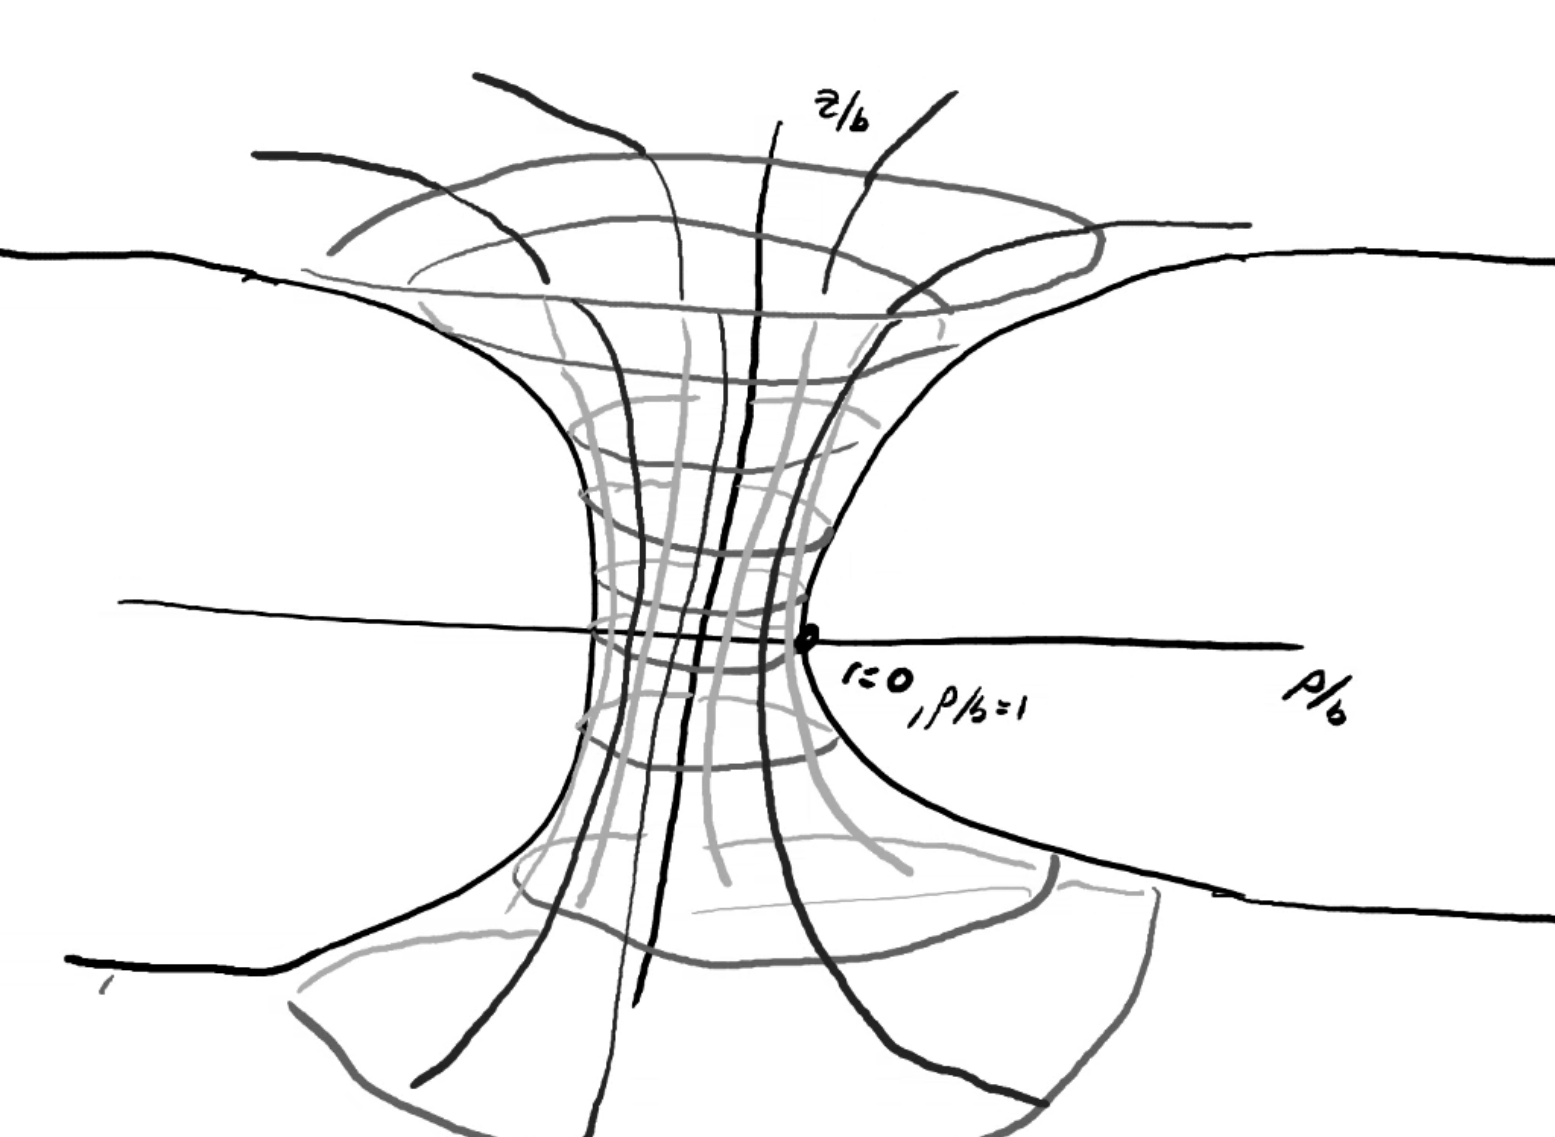
\includegraphics[width = 0.6\textwidth]{Figures/Ch7/wormhole.png}
\end{center}
\caption{Wormhole Embedding}\label{fig:wormhole}
\end{figure}

We note that when \(r=0\) we have \(\rho/b = 1\) and we are at the neck of the wormhole

\subsubsection{Geodesics}
We can of course compute the geodesic equations by taking the variation of the lagrangian:
\begin{subequations}
	\begin{equation}
		\der{t}{\tau2} = 0\label{eq7:wh1}
	\end{equation}
	\begin{equation}
		\der{r}{\tau2} = r\left[\left(\der{\theta}{\tau}\right)^2 + \sin^2\theta\left(\der{\theta}{\tau}\right)^2\right]\label{eq7:wh2}
	\end{equation}
	\begin{equation}
		\der{}{\tau}\left[\left(b^2 + r^2\right)\der{\theta}{\tau}\right] = \left(b^2+r^2\right)\sin\theta\cos\theta\left(\der{\phi}{\tau}\right)^2\label{eq7:wh3}
	\end{equation}
	\begin{equation}
		\der{}{\tau}\left[\left(b^2+r^2\right)\sin^2\theta\der{\phi}{\tau}\right] = 0\label{eq7:wh4}
	\end{equation}
\end{subequations}
Consider a particle in free motion radially, that is
\[u^\alpha = (u^t, u^r, u^\theta, u^\phi) = (C,U,0,0)\]
Normalizing the 4-velocity, we find
\[u^\alpha = \left((1-U^2)^{1/2},U,0,0\right)\]
Because \(u^\theta = u^\phi = 0\) we find Equation~\ref{eq7:wh2} becomes
\[\der{r}{\tau2} = \der{u^r}{\tau} = 0\]
so
\[r(\tau) = U\tau +R\]
and so to get from one side of the wormhole to the other,
\[\Delta\tau = \frac{2R}{U}\]

\section{Symmetries and Conservation}
Recall Noether's theorem: suppose \(L\) remains invariant under a certain coordinate transformation. Then, every such transformation there exists a conserved quantity. However, our lagrangian is in terms of the metric, and so we must find a new way to extract symmetries.
\section{Killing Vectors}
We can reformulate Noether's theorem using the metric and geodesic equation. Consider the line element
\[\d{s}^2 = \d{x}^2 + \d{y}^2 + \d{z}^2\]
for flat spacetime. This metric doesn't depend on any of \(x,y,z\), and so our metric has \emph{translational symmetry}. 

We define a \emph{Killing vector field} which is a vector field that points along a direction where the metric remains invariant.
Three components of the Killing field correspond to the translational symmetry:
\[\xi^1= (1,0,0)\]
\[\xi^2= (0,1,0)\]
\[\xi^3= (0,0,1)\]
More explicity, for a symmetry along \(x^\sigma\), we have a Killing vector
\[\Sigma^\mu = (\partial_\sigma)^\mu\]
and three components correspond to the rotational symmetry. This metric is \emph{maximally symmetric} because these six degrees of freedom are the maximum number of symmetries in 3D space. In 4D space time, there are a maximum of 10 symmetries, corresponding to the 10 degrees of freedom in the Poincar\'e group.

We see that if the metric is independent of a coordinate, say \(x^1\), we find
\[\pder{L}{x^1} = 0\]
so
\[\pder{L}{\left(\der{x^1}{\sigma}\right)} = \text{const}\]
Rewriting the LHS, we have
\[\pder{L}{\left(\der{x^1}{\sigma}\right)}=-g_{1\beta}\frac{1}{L} \der{x^\beta}{\sigma} = -g_{1\beta}\der{x^\beta}{\tau}\]
We see that because \(\xi^1 = (1,0,0)\), we can insert it into the equation to find
\[-\xi^1* u  = \text{const}\]
more generally,
\begin{equation}
	\xi*p = \text{const}
\end{equation}
or momentum along a killing vector is conserved. In cartesian coordinates, we have then the momentum along translations is conserved, or linear momentum, and that momentum along rotations is conserved, or angular momentum.

Another example, is using polar coordinates
\[g_{AB} = \begin{pmatrix}
	1 & 0 \\ 0 & r^2
\end{pmatrix}\]
we find a killing vector
\[\xi = (0,1)\]
We find then, that we have a conserved quantity
\[\ell =\xi* u = g_{AB}\xi^A u^B = r^2\der{\phi}{s}\]
From the normalization of the velocity,
\[\left(\der{r}{s}\right)^2 = 1 - r^2\left(\der{\phi}{s}\right)^2 = 1-\frac{1}{r^2}\left(r^2\der\phi s\right)^2 = 1-\frac{\ell^2}{r^2}\]
With an appropriate choice of coordinates, we can then extract a geodesic equation.

\section{Motion in a static isotropic spacetime}
Consider the Schwarzschild metric
\begin{equation}
	\d{s}^2 = -\left(1-\frac{2GM}{c^2 r}\right)(c\d{t})^2 + \left(1-\frac{2GM}{c^2 r}\right)^{-1}\d{r}^2 + r^2 \left(\d\theta^2 + \sin^2\theta\d\phi^2\right)
\end{equation}
This is a \emph{static} metric, meaning there is no time dependence. Further, we impose spherical symmetry, given by \(g_{\theta\theta}\) and \(g_{\phi\phi}\). Note, the spherical symmetry is sometimes written using
\[\d\Omega^2 = \d\theta^2 + \sin^2\d\phi^2\]
We can thus extract the two killing vectors
\[\xi^\mu = (1,0,0,0)\]
\[\eta^\mu = (0,0,0,1)\]
Our first conserved quantity is given (in planck natural units \(c=G=\hbar=k_B=1\))
\[e = -\xi* u = g_{tt}\der{t}{\tau} = \left(1-\frac{2M}{r}\right)\der{t}{\tau}\]
\[\ell = -\eta * u = r^2\sin^2\theta\der\phi\tau\]
\[u*u = -1\]
We denote these \(e\) and \(\ell\), as they are akin to an energy and angular momentum, each per unit mass.

\subsection{Effective Potential}
Just like in the two-body problem in classical mechanics, we will consider the orbits in an effective potential. Note that from conservation of \(\ell\), we know that the particle must have a planar orbit. We can fix then \(\theta = \pi/2\) and \(u^\theta = 0\). Using the normalization of velocity,
\[-1 = - \left(1-\frac{2M}{r}\right) \left(\der{t}{\tau}\right)^2 + \left(1-\frac{2M}{r}\right)^{-1}\left(\der{r}{\tau}\right)^2 + r^2\left(\der{\phi}{\tau}\right)^2\]
Plugging in our conserved quantities,
\[1 = -\left(1-\frac{2M}{r}\right)^{-1}e^2 + \left(1-\frac{2M}{r}\right)^{-1}\left(\der{r}{\tau}\right)^2 + \frac{\ell^2}{r^2}\]
Rearranging, we find
\[\frac{e^2-1}{2} = \frac{1}{2}\left(\der{r}{t}\right)^2 + \frac{1}{2}\left[\left(1-\frac{2M}{r}\right)\left(1+\frac{\ell^2}{r^2}-1\right)\right]\]
Note that because the LHS is a constant, the RHS is also constant. We redefine \(\mathcal{E} = \frac{e^2-1}{2}\). We identify the first term on the RHS as the kinetic energy per unit mass, and the second term as \(V_{eff}\), the effective potential. Expanding, we find
\[V_{eff} = -\frac{M}{r} + \frac{\ell^2}{2r^2} -\frac{M\ell^2}{r^3}\]
We then identify the first term in the effective potential as the gravitational potential and the second as the centrifugal barrier. Howerver, we obtain a third, new term in the effective potential. Thus we obtain
\[\mathcal{E} = \frac{1}{2}\left(\der{r}{\tau}\right)^2 + V_{eff}(r)\]
which we can solve as in classical mechanics.

If we plot the effective potential, as in Figure~\ref{fig:veff}
\begin{figure}
\begin{center}
	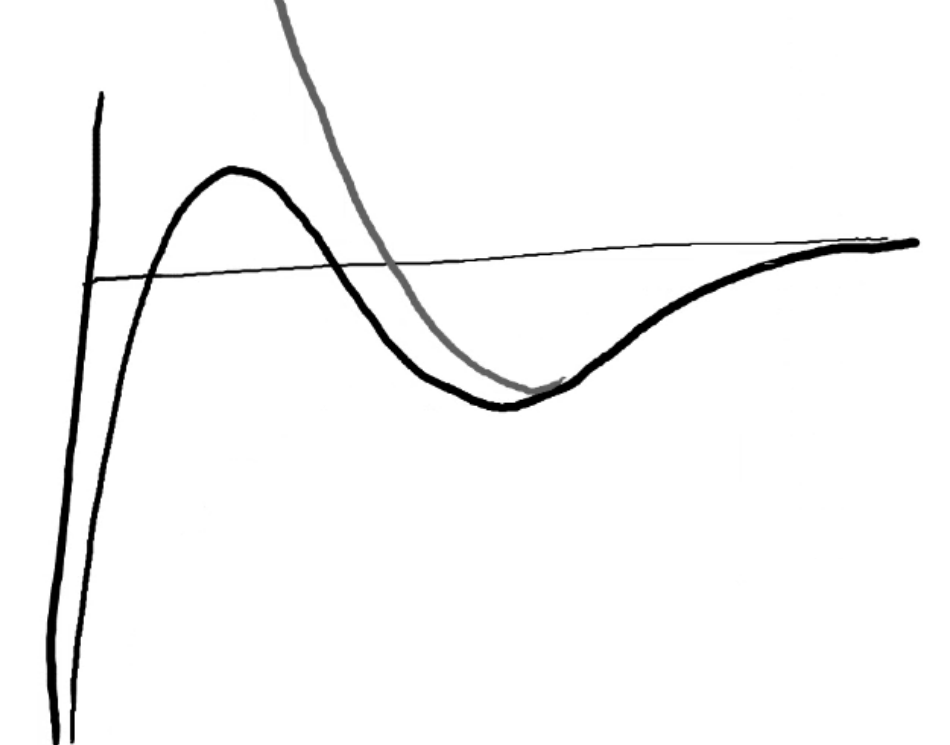
\includegraphics[width = 0.6\textwidth]{Figures/Ch7/veff.png}
\end{center}
\caption{Effective Potential}\label{fig:veff}
\end{figure}
we see there is a new unstable circular orbit. Less than this unstable orbit, the particle is pulled to the origin. Additionally, the minimum bound orbit is closer to the centre than classically expected.

Finding the extrema, we find
\[Mr^2 - \ell^2 r + 3M\ell = 0\]
so
\[r_{\min{},\max} = \frac{\ell}{2M}\left[1\pm\sqrt{1-12\left(\frac{M}{\ell}\right)^2}\right]\]
We see there is then a critical \(\ell_c\) where the stable and unstable orbit coincide:
\[\frac{\ell_c}{M} = \sqrt{12}\]
We also have a special radius, the Schwarzschild radius, where the metric becomes singular:
\[r_s = 2M\]
these two values are related by 
\[\frac{\ell_c}{r_s} = \sqrt{3}\]

\subsection{Plunging Orbits}
\[\der{t}{\tau} = \frac{e}{1-\frac{r_s}{r}}\]

\subsection{Elliprical Orbit}
Recall by definition that
\[\der{\phi}{\tau} = \frac{\ell}{r^2}\]
so
\[\der{r}{\tau} = \der{r}{\phi}\der{\phi}{\tau} = \der{r}{\phi}\frac{\ell}{2}\]
thus, we can integrate
\[\phi(r) = \pm \int\d{r}\frac{\ell}{r^2\sqrt{\mathcal{E}^2 - 2V(r)}}\]
Upon integration, we find that the perihelion precesses.

Consider the tangent of the embedding of the schwarzschild metric into \(\R^3\). If we revolve this tangent around, it forms a cone; however to form this cone into flat spacetime, we need to add an angular sliver; this angular sliver corresponds to the precession. Define
\[\tan\alpha = \der{z}{r}\]
we then have
\[(2\pi-\delta)R = 2\pi r = 2\pi R\cos\alpha\]
for \(r\gg 2M\), we can use the small angle approximation, so
\[\delta = \frac{2\pi M}{r} = \frac{1}{3}\frac{6\pi M}{r}\]
which is about a third of the orbit in flat space.
\subsection{Bound Orbits}
Just as in classical mechanics, we make the substitution
\[u = r^{-1}\]
so we can find
\[\der{r}{\phi} = \frac{1}{u^2}\d{u}{\phi}\]
and 
\[\der{\phi}{\tau} =\ell u^2\]
so we can rewrite our orbital equation as
\[\mathcal E = \frac{1}{2}\left(-\frac{1}{u^2}\der{u}{\phi}\right)^2\ell u^4 - Mu +\frac{1}{2}\ell^2 u^2 - M\ell^2 u^3\]

There is an innermost stable circular orbit, given by
\[r_{\text{ISCO}} = 6M = 3r_2\]
which is were the minimum coincides with the maximum in the potential. 

We find that if we send a particle from \(r=\infty\) to the innermost stable circular orbit, a particle will release 6\% of its energy (eventually to radiation)\footnote{Quadrupole moments are required to generate gravitational waves, however, so perfectly circular orbits will not radiate away}. Compared to nuclear fusion, which releasees only 0.7\%, this is immense\footnote{Rotating black holes can further increase this efficiency to around 40\%!}.

\section{Bending of Light}
Recall that light follows null geodesics, so
\[u*u = g_{\alpha\beta}\der{x^\alpha}{\lambda}\der{x^\beta}{\lambda} = 0\]
This allows us to rewrite conserved quantities
\[e = -\xi*u = \left(1-\frac{2M}{r}\right)\der{t}{\lambda}\]
\[\ell = -\eta*u = r^2\sin^2\theta\der{\phi}{\lambda}\]
\[u*u = -\left(1-\frac{2M}{r}\right)\left(\der{t}{\lambda}\right)^2 + \left(1-\frac{2M}{r}\right)\left(\der{r}{\lambda}\right)^2 + r^2\left(\der{\phi}{\lambda}\right) = 0\]
so
\[\frac{1}{b^2}\equiv\frac{e^2}{\ell^2}= \frac{1}{\ell^2} \left(\der{r}{\lambda}\right)^2 + \frac{1}{r^2}\left(1-\frac{2M}{r}\right)\]
for the \emph{impact parameter}, \(b\).
We can the write
\[\frac{1}{b^2} = \frac{1}{\ell^2}\left(\der{r}{\lambda}\right)^2 + W_{eff}\]
for the effective potential \(W_{eff}\). Now, our effective potential for light is slightly different than for a particle.
\[W_{eff} = \frac{1}{r^2}\left(1-\frac{2M}{r}\right)\]
we find there is a single circular orbit at
\[r = 3M\]
but no stable bound orbits. At this point, the impact parameter is given 
\[\frac{1}{b^2} = \frac{1}{27M^2}\]
for \(r>3M\), we have \emph{scattering}, where
\[\frac{1}{b^2}<\frac{1}{27M^2}\]
and the photon is deflected, and for \(r<3M\) we have the photon captured by the singularity.

For \(r=2M\), we are at the \emph{event horizon}, where light can only escape if it travels radially outward. 

Once again rewriting in terms of \(u =1/r\), we find
\[\der{u}{\phi2}+u = 3Mu^2\]
and can compute the bending of light around a mass.
